\documentclass[12pt, a4paper, oneside]{ctexbook}
\usepackage{amsmath, amsthm, amssymb, bm, wallpaper}
\usepackage{graphicx, hyperref, mathrsfs, caption}
\usepackage{float, subfigure, enumerate, ulem, paralist}
\usepackage{cite, listings, color}


\CTEXsetup[format={\Large\bfseries}]{section}
\linespread{1.5}
\newtheorem{theorem}{定理}[section]
\newtheorem{definition}[theorem]{定义}
\newtheorem{lemma}[theorem]{引理}
\newtheorem{corollary}[theorem]{推论}
\newtheorem{example}[theorem]{例}
\newtheorem{proposition}[theorem]{命题}

\newcommand\zm[2]{\begin{proof}[\textbf{#1}]
    #2
\end{proof}}
\newcommand\jie[2]{\begin{proof}[\textbf{#1}]
    #2
\end{proof}}
\newcommand\bv[1]{\boldsymbol{#1}}
\newcommand\mb[1]{\mathbb{#1}}
\newcommand\mc[1]{\mathcal{#1}}

% \renewcommand{\qedsymbol}{}

\captionsetup{labelformat=default,labelsep=space} %去除冒号

\begin{document}

\title{{\Huge{\textbf{Time Series Analysis}}\\}}
\author{Lollins}
\date{\today}

\maketitle

\pagenumbering{roman}
\setcounter{page}{1}

\begin{center}
    \Huge\textbf{前言}
\end{center}
\par 时间序列分析的笔记,图像大多用Python完成,源代码放在code文件夹下。


\begin{flushright}
    \begin{tabular}{c}
        Lollins \\
        \today
    \end{tabular}
\end{flushright}

\newpage
\pagenumbering{Roman}
\setcounter{page}{1}
\tableofcontents
\newpage
\setcounter{page}{1}
\pagenumbering{arabic}

\chapter{时间序列分析简介}
\section{时间序列的定义}
\subsection{随机过程中的一些基本定义}
\begin{definition}[概率空间]
    $(\Omega,\mathcal{F},\mc{P})$称为概率空间当且仅当其满足以下的条件:
    \begin{enumerate}[1.]
        \item $\Omega$-Simple Space样本空间,试验中所有可能结果的集合。
        \item $\mc{F}$-Sets of events事件集合,是$\Omega$子集构成的集合,即$\mc{F} \subset 2^{\Omega}(\Omega\text{的幂集})$
              ,并且它需要满足以下三个特征$\left(\text{也就是必须是}\sigma-field\right)$:
              \begin{itemize}
                  \item $\Phi \subset \mc{F}\left(\text{即必须包含不可能事件}\right)$;
                  \item 如果$A \subset \mc{F}$,那么$A^c \subset \mc{F}$;
                  \item 如果$A_{1},A_{2},\ldots,A_{i}\in\mathcal{F},\text{那么}\bigcup_{i=1}^{\infty}A_{i}\in\mathcal{F}$.
              \end{itemize}
        \item $\mc{P}$-Probability measure概率测度$\left(\text{或概率}\right)$,描述一次随机试验中被
              包含在$\mc{F}$中的所有事件的可能性。并且它也类似的需要满足以下三个特征:
              \begin{itemize}
                  \item $0\leq \mc{P}(A)\leq1$,即限制了总测度为1;
                  \item $\mc{P}(\Omega)=1$,即包含样本空间且概率为1;
                  \item 如果$A_{1},A_{2},\ldots,A_{i}$为互斥事件,那么$\mc{P}(\bigcup_{i=1}^{\infty}A_{i})
                            = \sum_{i=1}^{\infty}\mc{P}(A_i)$
              \end{itemize}
    \end{enumerate}
\end{definition}

\begin{definition}[随机过程]
    随机过程是概率空间$(\Omega,\mathcal{F},\mc{P})$上的一族随机变量$\{X(t),t \in T\}$,
    其中t是参数,它属于某个指标集T,T称为参数集。
\end{definition}
\textbf{注:}依据参数集$T$可分为\textbf{离散参数过程}和\textbf{连续参数过程},把\textbf{离散参数过程}称为\textbf{随机序列}。
\subsection{随机序列定义}
\begin{definition}[随机序列]
    按时间顺序排列的一组随机变量
    \begin{equation*}
        \ldots,X_1,X_2,\ldots,X_{t},\ldots
    \end{equation*}
\end{definition}

\begin{definition}[观察值序列]
    随机序列的n个有效观察值,称之为序列长度为n的观察值序列
    \begin{equation*}
        x_1,x_2,\ldots,x_{n}
    \end{equation*}
\end{definition}

\subsubsection{随机序列与观察值序列的关系}
\begin{itemize}
    \item 观察值序列是随机序列的一个实现;
    \item 通过分析观察值序列的性质,由观察值序列的性质来推断随机序列的性质.
\end{itemize}

\subsubsection*{随机序列的特点}
\begin{itemize}
    \item 随机序列中数据的位置与实践有关;
    \item 时间序列是对相关指标变量在不同时间进行观察所得到的结果。是一个观察结果,一个实现;
    \item 时间序列中的数据可以是一个时期内的数据也可以是一个时点上的数据。流量与存量;
    \item 时间序列通常存在前后时间上的相依性.
\end{itemize}

\subsubsection*{时间序列的分类}
\begin{itemize}
    \item 按所研究对象的维度,有一元时间序列和多元时间序列;
    \item 按观察时间的连续与否可将时间序列分为离散时间序列和连续时间序列;
    \item 按时间序列的统计特征分,有平稳时间序列和非平稳时间序列两类.
\end{itemize}

\subsubsection*{时间序列分析的目的}
时间序列分析所讨论的内容,就是对观察到的时间序列数据进行研究,分析时间序列的统计
特征和依存关系,找出系统的内在发展规律,建立起能反映变量变化的动态模型,并将这种
动态模型用于预测等应用领域.

\section{时间序列分析方法}
\subsection{描述性时间序列分析}

\subsection{统计时间序列分析}
\begin{equation*}
    \left\{ \begin{array}{l}
        \text{频域分析方法} \\
        \text{时域分析方法}
    \end{array} \right.
\end{equation*}

\section{时间序列分析软件}
Matlab,Eviews,R和SAS等。

\chapter{时间序列的预处理}
\section{平稳序列的定义}
\subsection{特征统计量}
\subsubsection{一、概率分布}
\subsubsection{概率分布的意义}
随机变量族的统计特征完全由它们的联合分布函数或联合密度函数决定。
\begin{definition}[时间序列概率分布族]
    对于时间序列$\{X_t,t \in T\}$,任取正整数m,任取$t_1,t_2,\cdots,t_m\in T$,
    则m维随机向量$(X_1,X_2,\cdots,X_m)'$的联合概率分布记为$F_{t_1,t_2,\cdots,t_m}(x_1,x_2,\cdots,x_m)$,
    由这些有限维分布函数构成的全体
    \begin{equation}
        \left\{F_{t_1,t_2,\cdots,t_m}(x_1,x_2,\cdots,x_m),\forall m\in N,\forall t_1,t_2,\cdots,t_m\in T\right\}
    \end{equation}
    \par 就称为序列$\{X_t\}$的概率分布族。
\end{definition}
\textbf{注:}默认$t$为正整数。


\subsubsection{实际应用的局限性}
在实际应用中, 要得到序列的联合概率分布几乎是不可能的, 而且联合概率分布通常涉及非常复杂的数学运算, 这些原因导致我们很少直接使用联合概率分布进行时间序列分析。

\subsubsection{二、特征统计量}
\begin{itemize}
    \item \textbf{均值:} $\mu_t=EX_t=\int_{-\infty}^\infty xdF_t(x)$
    \item \textbf{方差:} $DX_t=E(X_t-\mu_t)^2=\int_{-\infty}^\infty(x-\mu_t)^2dF_t(x)$
    \item  \textbf{自协方差:} $\gamma(t,s)=E(X_t-\mu_t)(X_s-\mu_s)$
    \item  \textbf{自相关系数:} $\rho(t,s)=\frac{\gamma(t,s)}{\sqrt{DX_t\cdot DX_s}}$
\end{itemize}

\textbf{注:}$\gamma(s,t)=\gamma(t,s)\text{,}|\rho(t,s)| \leq 1 $

\subsection{平稳时间序列的定义}
\subsubsection{一、严平稳}
严平稳是一种条件比较苛刻的平稳性定义,它认为只有当序列所有的统计性质都不会随着时间的推移而发生变化时,该序列才能被认为平稳。
\begin{definition}[严平稳]
    设$\{X_t\}$为一时间序列,对$\forall$正整数m,$\forall t_1,t_2,\cdots,t_m\in T\text{,}\forall\text{正整数}\tau$,有
    \begin{equation}
        F_{t_1,t_2\cdots t_m}\left(x_1,x_2,\cdots,x_m\right)=F_{t_{1+\tau},t_{2+\tau}\cdots t_{m+\tau}}\left(x_1,x_2,\cdots,x_m\right)
    \end{equation}
    \par 则称时间序列$\{X_t\}$为严平稳时间序列。
\end{definition}

\subsubsection{二、宽平稳}
宽平稳是使用序列的特征统计量来定义的一种平稳性。它认为序列的统计性质主要由它的低阶矩决定,所以只要保证序列低阶矩平稳(二阶),就能保证序列的主要性质近似稳定。

\begin{definition}[宽平稳]
    设$\{X_t\}$为一时间序列,若满足以下条件
    \begin{enumerate}[1.]
        \item $EX_t^2<\infty,\forall t\in T$
        \item $EX_t=\mu,\mu\text{为常数,}\forall t\in T$
        \item $\gamma(t,s)=\gamma(k,k+s-t),\quad\forall t,s,k\text{且}k+s-t\in T$
    \end{enumerate}
    \par 则称时间序列$\{X_t\}$为宽平稳时间序列。
\end{definition}

\subsubsection{三、严平稳与宽平稳的关系}
\begin{equation*}
    \left\{ \begin{array}{l}
        \text{严平稳} \nRightarrow  \text{宽平稳}            \\
        \text{严平稳} \nLeftarrow  \text{宽平稳}             \\
        \text{严平稳+二阶矩存在}  \Rightarrow  \text{宽平稳} \\
        \text{在正态分布假设下,(严平稳} \Leftrightarrow \text{宽平稳})
    \end{array} \right.
\end{equation*}

\textbf{注:}以后见到的平稳时间序列,如果没有特别注明,都是\textbf{宽平稳时间序列}。如果序列不满足平稳条件,就称为\textbf{非平稳时间序列}。
\begin{example}[白噪声序列(White Noise)]
    一个简单的随机时间序列是一具有零均值同方差的独立分布序列:$X_t=\mu_t,\mu_t\sim N(0,\sigma^2)$.
\end{example}
\jie{解}{由于$X_t$具有相同的均值和方差,且协方差等于0,有定义可以得到\textbf{白噪声序列是平稳的}}

\begin{example}[随机游走序列(Random Walk)]
    该随机时间序列是由随机过程$X_t=X_{t-1}+\mu_t$生成,其中$\mu_t$是一个白噪声序列.
\end{example}
\jie{解}{由$\mu_t \sim N(0,\sigma^2)$,我们可以知道该序列的均值满足
    \begin{equation*}
        E(X_t) = E(X_{t-1}) + E(\mu_t) = E(X_{t-1})
    \end{equation*}
    \par 我们设序列$X_t$的初值为常数$X_0$,则
    \begin{equation*}
        \begin{aligned}
            X_1    & = X_0 + \mu_1                       \\
            X_2    & = X_1 + \mu_2 = X_0 + \mu_1 + \mu_2 \\
            \cdots & = \cdots                            \\
            X_t    & = X_0 + \sum_{i=1}^{t}\mu_i
        \end{aligned}
    \end{equation*}

    由于$X_0$为常数,$\mu_t$为一个白噪声,所以$Var(X_t)=t\sigma^2$

    即$X_t$的方差和时间有关而非常数,它是一个\textbf{非平稳序列}.
}
\subsection{平稳时间序列的统计性质}
\subsubsection{一、常数均值}
\begin{equation}
    EX_t = \mu,\forall t \in T
\end{equation}
\subsubsection{二、自协方差函数和自相关系数只依赖于时间的平移长度而与时间的起止点无关}
\begin{itemize}
    \item 延迟$k$自协方差函数
          \begin{equation}
              \gamma(k)=\gamma(t,t+k),\forall k\text{为整数}
          \end{equation}
    \item 延迟$k$自相关系数
          \begin{equation}\label{eq2.5}
              \rho_k=\frac{\gamma(k)}{\gamma(0)}
          \end{equation}
\end{itemize}

由式\ref{eq2.5},我们可以得到\textbf{自相关系数}的如下性质:
\begin{itemize}
    \item \textbf{规范性:} $\rho_0=1,\text{且}|\rho_k|\leq1,\forall k$;
    \item \textbf{对称性:}$\rho_k=\rho_{-k}$;
    \item \textbf{非负定性:}$\begin{aligned}
                  \Gamma_m= & \begin{pmatrix}
                                  \rho_0     & \rho_1     & \cdots & \rho_{m-1} \\
                                  \rho_1     & \rho_0     & \cdots & \rho_{m-2} \\
                                  \vdots     & \vdots     & \cdots & \vdots     \\
                                  \rho_{m-1} & \rho_{m-2} & \cdots & \rho_0
                              \end{pmatrix},\Gamma_m\text{为非负定自协方差系数阵};
              \end{aligned}$
    \item \textbf{非唯一性:}一个平稳时间序列一定唯一决定了它的自相关系数,但一个自相关系数未必唯一对应着一个平稳时间序列.
\end{itemize}

\begin{example}[平稳序列的线性变换]
    平稳序列$\{X_t\}$,期望$\mu$,自协方差函数$\gamma(t)$,经线性变化后,还是平稳序列。
\end{example}
\zm{证明}{令$Y_t=a+bX_t$,则$EY_t=a+b\mu$,$\mathrm{Cov}(Y_s,Y_{s+t})=b^2\mathrm{Cov}(X_s,X_{s+t})=
        b^2\gamma(t)$,可见$\{Y_t\}$平稳。若取
    \begin{equation*}
        Y_t=\frac{X_t-\mu}{\sqrt{\gamma_0}}
    \end{equation*}
    则$EY_t=0,\operatorname{Var}(Y_t)=1$,称$\{Y_t\}$为$\{X_t\}$的标准化序列。
}

\begin{example}[调和平稳序列]\label{ex2.1.7}
    设a,b为常数,随机变量U在$(-\pi,\pi)$内均匀分布,则
    \begin{equation*}
        X_t=bcos(at+U),t \in \mb{Z}
    \end{equation*}
    是平稳序列,称为调和平稳序列。
\end{example}
\zm{证明}{
    \begin{equation*}
        \begin{aligned}
            EX_{t}        & =\frac{1}{2\pi}\int_{-\pi}^{\pi}b\cos(at+u)du=0,            \\
            E(X_{t}X_{s}) & =\frac{1}{2\pi}\int_{-\pi}^{\pi}b^{2}\cos(at+u)\cos(as+u)du \\
                          & =\frac12b^2\cos((t-s)a),
        \end{aligned}
    \end{equation*}
    证毕!
}

\subsection{平稳性的重大意义}
\begin{itemize}
    \item 在平稳序列场合,序列的均值等于常数,这意味着原本含有可列多个随机变量的均值序列变成了只含有一个变量的常数序列。
          \begin{equation}
              \{\mu_t,t\in T\}\Rightarrow\{\mu,t\in T\}
          \end{equation}
    \item 原本每个随机变量的均值(方差,自相关系数)只能依靠唯一的一个样本观察值去估计,现在由于平稳性,每一个统计量都将拥有大量的样本观察值。
    \item 这极大地减少了随机变量的个数,并增加了待估变量的样本容量。极大地简化了时序分析的难度,同时也提高了对特征统计量的估计精度。
\end{itemize}

\section{序列的平稳性检验}
检验的方法分为\textbf{图检验}与\textbf{构造检验统计量进行假设检验}。

图检验分为时序图检验和自相关图检验。
\subsection{时序图检验}
得到观察值序列后,我们绘制该序列的时序图,根据时序图的不同特征,可以把序列分为三大类。
\subsubsection{1、序列具有明显的趋势特征}
如果序列具有明显的趋势特征,那么该序列显然不具有常数均值,所以趋势序列可以判断为非平稳。
\begin{example}
    图\ref{im2_1}时序图显示:序列有明显的递增趋势特征,所以是非平稳序列。
    \begin{figure}[h]
        \centering
        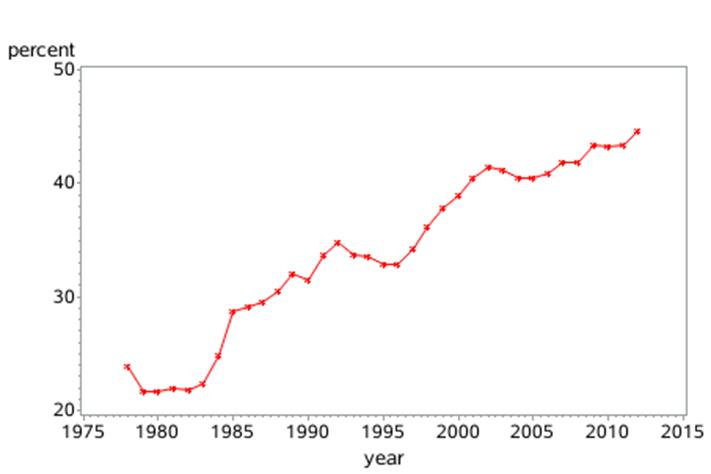
\includegraphics[scale = 0.6]{img/2_1.png}
        \caption{1978-2012年我国第三产业占国内生产总值}
        \label{im2_1}
    \end{figure}
\end{example}

\subsubsection{2、序列具有明显的周期特征}
具有周期特征的序列平稳性识别是困难的。理论上,如果周期波动的振幅和频率不随着时间的变化而变化,
通常序列是平稳的,例如例\ref{ex2.1.7}中的调和平稳序列。但是如果
$X_t=b_tcos(a_tt+U)$,振幅和频率随着时间的变化而变化,那么序列$\{X_t\}$
就是非平稳序列。

\subsubsection{3、序列既没有趋势特征,也没有周期特征}
如果一个序列既没有明显的趋势特征,也没有明显的周期特征,几乎是围绕着一个常数附近做有解波动,这通常是平稳序列。

\subsection{自相关图检验}
\begin{example}
    利用图检验方法判断1915-2004年澳大利亚自杀率序列(每10万人自杀人口数)的平稳性,如图\ref{im2_2}所示。
    \begin{figure}[h]
        \centering
        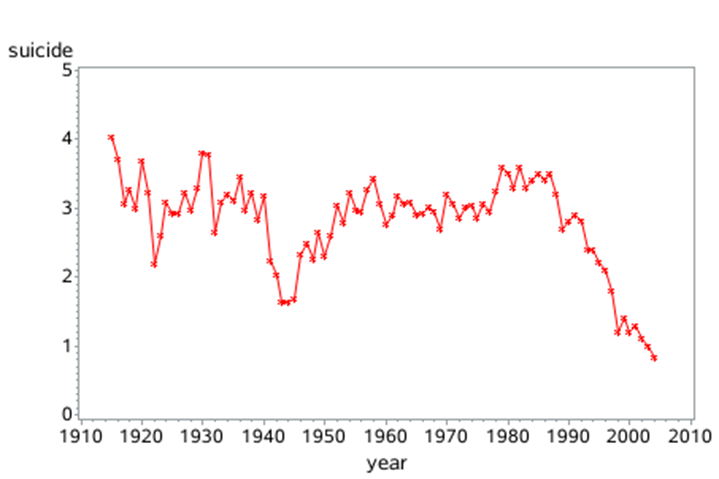
\includegraphics[scale=0.6]{img/2_2.png}
        \caption{}
        \label{im2_2}
    \end{figure}
\end{example}
图\ref{im2_2}难以把握该序列的平稳性,我们可以借助自相关图的性质来进一步辅助判别。

Python中可以用statsmodels库来绘制自相关图,如图\ref{im2_3}所示。
\begin{figure}[h]
    \centering
    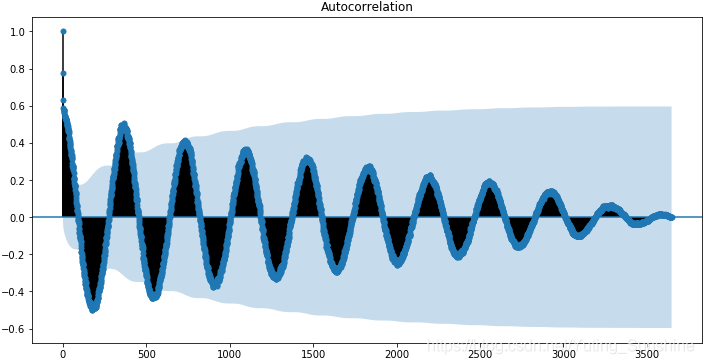
\includegraphics[scale=0.4]{img/2_3.png}
    \caption{}
    \label{im2_3}
\end{figure}

\textbf{自相关图}是一个平面二维坐标悬垂线图,横坐标表示延迟时期数,纵坐标表示自相关系数,
悬垂线的长度表示自相关系数的大小。

\subsubsection{1、序列具有明显的趋势特征}
该序列的时序图与自相关图如图\ref{im2_4}所示,自相关图呈现明显的倒三角特征,是非平稳序列,代码为\texttt{2\_4.py}。

\begin{figure}[ht]
    \centering
    \subfigure[时序图]{
        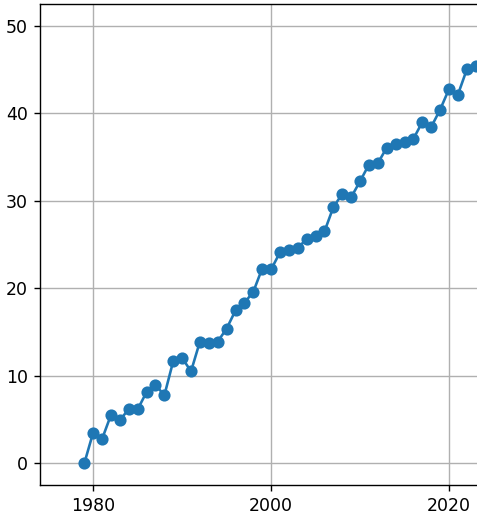
\includegraphics[width=0.45\textwidth]{img/2_4_1.png}
    }
    \hfill
    \subfigure[自相关图]{
        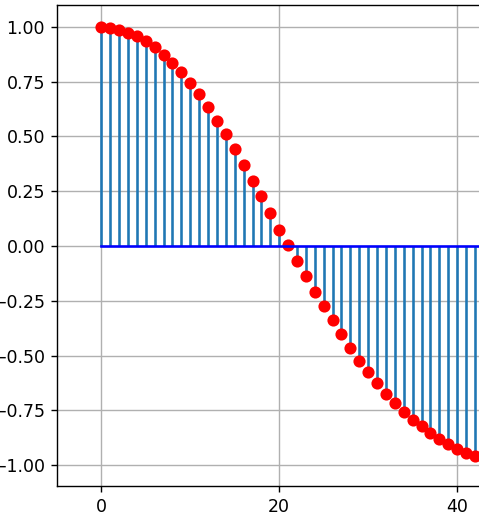
\includegraphics[width=0.45\textwidth]{img/2_4_2.png}
    }
    \caption{}
    \label{im2_4}
\end{figure}

\subsubsection{2、序列具有明显的周期特征}
该序列的时序图与自相关图如图\ref{im2_5}所示,自相关图呈现明显的周期特征,是非平稳序列,代码为\texttt{2\_5.py}。

\begin{figure}[hp]
    \centering
    \subfigure[时序图]{
        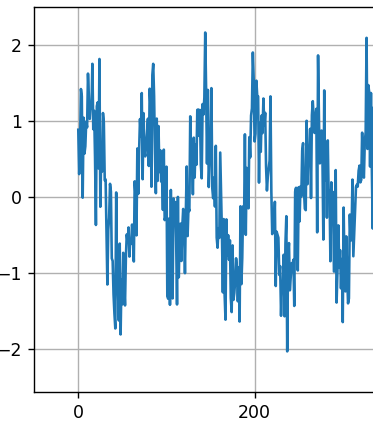
\includegraphics[width=0.45\textwidth]{img/2_5_1.png}
    }
    \hfill
    \subfigure[自相关图]{
        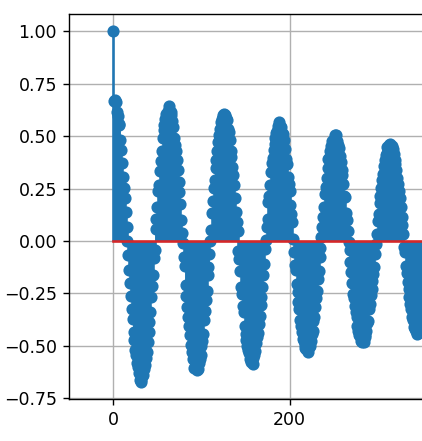
\includegraphics[width=0.45\textwidth]{img/2_5_2.png}
    }
    \caption{}
    \label{im2_5}
\end{figure}

对于有周期性的序列,平稳与非平稳时间序列的自相关图的图像很相像,但是平稳时间序列的自相关图随着之后(lag)的增加,
自相关系数减小的更快。从图\ref{im2_5a}中可以看出,代码为\texttt{2\_5a.py}。

\begin{figure}[hp]
    \centering
    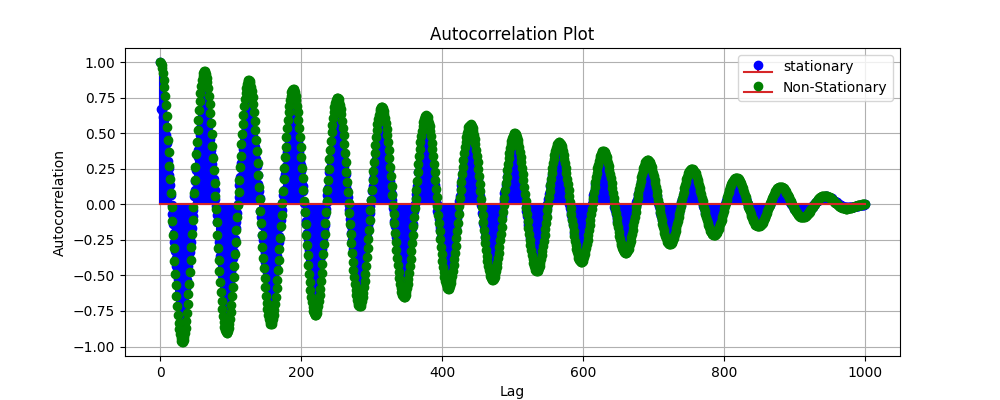
\includegraphics[scale = 0.6]{img/2_5a.png}
    \caption{蓝色为平稳时间序列,绿色为非平稳}
    \label{im2_5a}
\end{figure}

\subsubsection{3、平稳时间序列}
平稳时间序列的自相关图,除了0阶延迟为1,其余各阶自相关系数都很小,
而且自相关系数时正时负,没有倒三角特征,也没有周期特征,如图\ref{im2_6}所示,代码为\texttt{2\_6.py}。

\begin{figure}[h]
    \centering
    \subfigure[时序图]{
        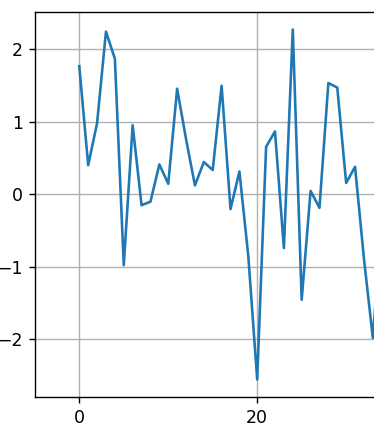
\includegraphics[width=0.45\textwidth]{img/2_6_1.png}
    }
    \hfill
    \subfigure[自相关图]{
        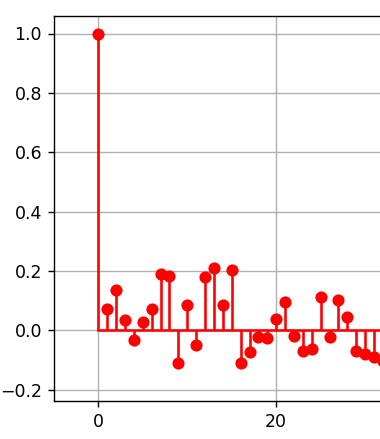
\includegraphics[width=0.45\textwidth]{img/2_6_2.png}
    }
    \caption{}
    \label{im2_6}
\end{figure}

\section{纯随机性检验}
拿到一个观察值序列后,首先判断它的平稳性。通过\textbf{平稳性检验},可以将序列分为\textbf{平稳和非平稳}。

对于平稳时间序列,我们有一套非常成熟的平稳序列建模方法。但是,并\textbf{不是所有的平稳时间序列都值得建模}。

如果序列值彼此之间没有任何相关性,那就意味着该序列是一个没有记忆的序列,
过去的行为对将来的发展没有丝毫影响,这种序列称为\textbf{纯随机序列}。
从统计分析的角度来说,纯随机序列是没有任何分析价值的序列。

\subsection{纯随机序列的定义}

\begin{definition}[白噪声(White Noise)序列]
    如果对于时间序列$\{X_t\}$满足以下性质:
    \begin{enumerate}[1、]
        \item 任取$t \in T$,有$E(X_t)=\mu$;
        \item 任取$t \in T$,有\begin{equation}
                  \gamma(t,s) = \begin{cases}
                      \sigma^2,t=s \\
                      0,t \neq s
                  \end{cases}
              \end{equation}
    \end{enumerate}
    称序列$\{X_t\}$为纯随机序列,也称为白噪声(White Noise)序列,简记为$X_t\sim WN(\mu,\sigma^2)$。
    容易证明,白噪声序列是平稳序列,而且是最简单的平稳序列。
\end{definition}

\subsection{纯随机序列的性质}
\subsubsection{1、纯随机性}
白噪声序列具有以下性质:
\begin{equation}\label{eq2.8}
    \gamma(k)=0,\forall ~k\neq 0
\end{equation}
这说明白噪声序列之间没有任何相关联系,这种“没有记忆”的序列就是\textbf{白噪声序列}。

如果序列值之间呈现出某种显著的相关分析:
\begin{equation}
    \gamma(k)\neq 0,\exists ~k\neq 0
\end{equation}
说明\textbf{该序列不是纯随机序列},该序列间隔k期之间存在一定程度的相互影响。

\subsubsection{2、方差齐性}
所谓的方差齐性,是指序列中每一个变量的方差都相等,即
\begin{equation}
    DX_t = \gamma(0)=\sigma^2
\end{equation}
如果序列不满足方差齐性,就称该序列具有\textbf{异方差性质}。

\subsection{纯随机性检验}\label{subse2.3.3}
如果一个序列是纯随机的,那么它的序列值之间应该没有任何相关关系,即式\ref{eq2.8}所示。

Bartlett证明,如果一个时间序列是纯随机的,得到一个观察期数为n的观察序列$\{x_t,~t = 1,2,...,n\}$,那么该序列的延迟非零期的样本自相关系数
将近服从均值为0,方差为序列观察期倒数的正态分布,即
\begin{equation}
    \hat{\rho_k} \overset{\bullet}{\operatorname*{\sim}} N(0,\frac{1}{n}),~\forall k \neq 0
\end{equation}
式中,n为序列观察期数。

根据Bartlett定理,我们可以构造检验统计量来检验序列的纯随机性。

\subsubsection{1、假设条件}
原假设:延迟期数小于或等于m期的序列值之间相互独立,即序列是延迟到m期都是平稳,纯随机的。

备择假设:延迟期数小于或等于m期的序列值之间有相关性。

该假设条件用数学语言描述为:
\begin{equation}
    \begin{aligned}
         & H_0:\rho_1=\rho_2=\cdots=\rho_m=0,\forall m\geqslant1                \\
         & H_1:\text{至少存在某个 }\rho_k\neq0,\forall m\geqslant1,k\leqslant m
    \end{aligned}
\end{equation}

\subsubsection{2、检验统计量}

\textbf{(1)Q统计量}

Box和Pierce推导出了Q统计量:
\begin{equation}
    Q=n\sum_{k\operatorname{=}1}^m\hat{\rho}_k^2\overset{\bullet}{\operatorname*{\sim}}\chi^2(m)
\end{equation}
n为序列观察期数,m为指定延迟期数。

\textbf{(2)LB统计量}

实际应用中,人们发现Q统计量在大样本场合检验效果很好,但在小样本场合不太准确。为了
弥补这一缺陷,Ljung和Box又推导了LB统计量
\begin{equation}
    LB=n(n+2)\sum_{k=1}^m\left(\frac{\hat{\rho}_k^2}{n-k}\right)
    \overset{\bullet}{\operatorname*{\sim}} \chi^2(m)
\end{equation}

以上(1)和(2)统计量的拒绝域都是$Q > \chi^2(m)_{1-\alpha}$。


\subsection{Eviews差分指令}
对序列$x_t$做差分,即
\begin{equation}
    y_t = x_t - x_{t-1}
\end{equation}
指令如下为genr y = D(x),同理,二阶差分为genr y = D(D(x))。

\chapter{ARMA模型的性质}

\section{Wold分解定理}
\subsection{Wold分解定理的内容}
\begin{definition}[Wold分解定理]
    对于任意一个离散平稳时间序列$\{x_t\}$,它都可以分解为两个不相关的平稳序列之和,
    其中一个为确定性的(deterministic),另一个为随机性的(stochastic),不妨记作:
    \begin{equation}
        x_t = V_t+ \xi_t
    \end{equation}
\end{definition}
确定性序列$\{V_t\}$代表序列的当期波动可以由其历史信息预测的部分。Wold证明,
平稳时间序列的确定性部分一定可以表达为历史序列值的线性组合:
\begin{equation}\label{eq3.2}
    V_t = \sum_{j = 1}^{\infty}\phi_jx_{t-j}
\end{equation}

随机序列$\{\xi_t\}$代表序列的当期波动不能由其历史信息预测的部分。Wold证明,
这部分信息可以等价表达为:
\begin{equation}\label{eq3.3}
    \xi_t = \sum_{j = 0}^{\infty}\theta_j\varepsilon_{t-j}
\end{equation}
式中,$\theta_0 = 1,\sum_{j = 0}^{\infty}\theta_j^2<\infty$,$\{\epsilon_t\}$称为新息过程(innovation process)
,是每个过程新加入的随机信息。$\varepsilon_t$为白噪声序列,序列值之间相互独立,不可预测,通常假定$\{\varepsilon_t\}
    \stackrel{i.i.d}{\sim}N(0,\sigma_{\varepsilon}^{2})$

具有式\ref{eq3.2}结构的模型是1927年Yalu提出的自回归(autoregression)模型,简称AR模型。
具有式\ref{eq3.3}结构的模型是1931年Walker提出的移动平均(moving average)模型,简称MA模型。



\section{AR模型}
\subsection{差分的定义}
\begin{itemize}
    \item 一阶差分:$\nabla x_t = x_t - x_{t-1}$
    \item p阶差分:$\nabla^p x_t = \nabla^{p-1} x_t - \nabla^{p-1} x_{t-1}$
    \item k步差分:$\nabla_k x_t = x_t - x_{t-k}$
\end{itemize}
定义B为一个延迟算子,即$B^p = x_{t-p}$,则我们有
\begin{itemize}
    \item 一阶差分:$\nabla x_t = (1-B)x_t$
    \item p阶差分:$\nabla^{p} x_t = (1-B)^{p}x_t$
    \item k步差分:$\nabla_k x_t = (1-B^k)x_t$
\end{itemize}

差分算子有如下性质:
\begin{enumerate}[1、]
    \item $B^0 = 1$;
    \item 常数的任意结束延迟仍然等于常数,即$B^p c = c$;
    \item 对于任意常数,有$B^p (cx_t) = cx_{t-p}$
    \item 对任意两个序列$\{x_t\},\{y_t\}$有$B(x_t \pm y_t) = x_{t-1} \pm y_{t-1}$
\end{enumerate}

关于差分方程的解法,可以参考周义仓老师的《差分方程及其应用》第二章的内容。

\subsection{AR模型的定义}
\begin{definition}
    具有如下结构的模型称为p阶自回归模型,简记为AR(p):
    \begin{equation}\label{eq3.4}
        \begin{cases}
            x_t=\phi_0+\phi_1x_{t-1}+\phi_2x_{t-2}+...+\phi_{p}x_{t-p}+\varepsilon_{t} \\
            \phi_p\neq0                                                                \\
            E(\varepsilon_{t})=0,\mathrm{Var}(\varepsilon_{t})=
            \sigma_{\varepsilon}^2,E(\varepsilon_t\varepsilon_{s})=0,s\neq t           \\
            E(x_s\varepsilon_{t})=0,\forall s<t
        \end{cases}
    \end{equation}
\end{definition}
AR(p)模型有三个限制条件:
\begin{enumerate}[1、]
    \item $\phi_p \neq 0$。保证模型的最高阶数为p。
    \item $E(\varepsilon_{t})=0,\mathrm{~Var}(\varepsilon_{t})=\sigma_{\varepsilon}^2,
              E(\varepsilon_t\varepsilon_{s})=0,s\neq t$。保证随机干扰项$\{\varepsilon_t\}$为零均值白噪声序列。
    \item $E(x_s\varepsilon_{t})=0,\forall s < t$。保证当期的随机干扰项与过去的序列值无关。
\end{enumerate}

当$\phi_0 = 0$,自回归模型又称为中性化AR(p)模型。非中心化AR(p)序列都可以通过下面的变换
转化为中心化AR(p)模型。令
\begin{equation}
    \mu=\frac{\phi_{0}}{1-\phi_{1}-\cdots-\phi_{p}},y_{t}=x_{t}-\mu
\end{equation}
则$\{y_t\}$为$\{x_t\}$的中心化序列。中心化序列就是将整个非中心化序列平移一个常数,
这个整体的移动对序列值之间的相关关系没有任何影响。

引入了延迟算子,中心化AR(p)模型又可以简记为
\begin{equation}
    \Phi(B)x_t = \varepsilon_t
\end{equation}
式中,$\Phi(B)=1-\phi_1B-\phi_2B^2-...-\phi_pB^p$,称为p阶自回归系数多项式。

\subsection{AR模型的平稳性判别}
并非所有的AR模型都是平稳的,图示法只是一种粗糙的直观判别方法,我们有两种准确的平稳性判断方法:
特征根判别法和平稳域判别。

\subsubsection{1、特征根判别法}
任一中心化AR(p)模型$\Phi(B)=\varepsilon_t$都可以视为一个非齐次线性差分方程
\begin{equation}
    x_{t}-\phi_{1}x_{t-1}-\phi_{2}x_{t-2}-...-\phi_{p}x_{t-p}=\varepsilon_{t}
\end{equation}
$\{x_t\}$平稳要求差分方程的特征根都在单位圆内,即
\begin{equation}
    |\lambda_i| < 1,~i=1,2,...,p
\end{equation}

\subsubsection{2、平稳域判别法}
从参数向量$(\phi_1,\phi_2,...,\phi_p)'$角度考虑,从p维欧氏空间取一个子集,满足:
\begin{equation*}
    \{\phi_1,\phi_2,\cdots,\phi_p|\text{ 特征根都在单位圆内 }\}
\end{equation*}
称为AR(p)模型的平稳域。

对于低阶AR模型,用平稳域的方法判别模型的平稳性通常更为简便。

\textbf{(1)AR(1)模型的平稳域}

AR(1)模型为:$x_t = \phi_1x_{t-1}+\varepsilon_t$,根据特征根判别法,可以求得
AR(1)模型的平稳域为$\{\phi_1|-1<\phi_1<1\}$

\textbf{(2)AR(2)模型的平稳域}

AR(2)模型为:$x_t = \phi_1x_{t-1}+\phi_2x_{t-2}+\varepsilon_t$,根据特征根判别法,可以求得
AR(2)模型的平稳域为$\{\phi_1,\phi_2|~|\phi_2|<1,\phi_2\pm \phi_1<1\}$

\subsection{平稳AR(p)模型性质}
\subsubsection{1、均值}
对于AR模型满足方程\ref{eq3.4},两边同时取期望
\begin{equation*}
    Ex_t=E(\phi_0+\phi_1x_{t-1}+\phi_2x_{t-2}+\cdots+\phi_px_{t-p}+\varepsilon_t)
\end{equation*}
根据平稳时间序列的常数均值性质,有$Ex_t = \mu~(\forall~t\in T)$,上式等价于
\begin{equation*}
    \begin{aligned}
                    & (1-\phi_1-\cdots-\phi_p)\mu=\phi_0        \\
        \Rightarrow & \mu=\frac{\phi_0}{1-\phi_1-\cdots-\phi_p}
    \end{aligned}
\end{equation*}
特别的,对于中心化AR(p)模型,$Ex_t=0$

\subsubsection{2、方差}
为求平稳AR(p)模型的方差,需要借助Green函数的帮助。
\begin{definition}[Green函数]
    假设$\{x_t\}$为任意阶数的平稳AR模型,那么一定存在一个常数序列$\{G_j\}(j=0,1,2...)$,使得
    $\{x_t\}$可以等价为纯随机序列$\{\varepsilon_t\}$的线性组合,即
    \begin{equation}\label{eq3.9}
        \begin{aligned}
            {x}_{t}
             & =\phi_1x_{t-1}+\phi_2x_{t-2}+\cdots+\phi_px_{t-p}+\varepsilon_t                                          \\
             & =G_0\boldsymbol{\varepsilon}_t+G_1\boldsymbol{\varepsilon}_{t-1}+G_2\boldsymbol{\varepsilon}_{t-2}\cdots
        \end{aligned}
    \end{equation}
    这个常数序列$\{G_j\}$就称为Green函数。
\end{definition}

基于Green函数,我们可以求出AR(p)模型的方差为
\begin{equation}
    Var(x_t)=\left(G_0^2+G_1^2+G_2^2+\cdots\right)\sigma_\varepsilon^2
\end{equation}

其中$G_j$满足(递推可求出)
\begin{equation}\label{eq3.11}
    \left.\left\{\begin{aligned}
        G_0 & =1                                                \\
        G_j & =\sum_{k=1}^j\phi_k^{\prime}G_{j-k},~j=1,2,\cdots
    \end{aligned}
    \right.\right.\text{式中}\phi_k^{\prime}=
    \begin{cases}\phi_k,k\leq p \\
        0,k>p &\end{cases}
\end{equation}

\begin{example}\label{ex3.2.3}
    求平稳AR(1)模型$x_t=\phi_1x_{t-1}+\varepsilon_t$,$\varepsilon_t\sim
        N(0,\sigma_{\varepsilon}^2)$的方差。
\end{example}
\jie{解}{
    根据式\ref{eq3.11},我们可以得到
    \begin{equation*}
        G_j=\begin{cases}
            1        & ,j=0          \\
            \phi_1^j & ,j=1,2,\cdots
        \end{cases}
    \end{equation*}
    再根据式\ref{eq3.9},得AR(1)模型的方差为
    \begin{equation*}
        Var(x_{t})=\sum_{j=0}^{\infty}G_{j}^{2}Var(\varepsilon_{t})
        =\sum_{j=0}^{\infty}\phi_{1}^{2j}\sigma_{\varepsilon}^{2}
        =\frac{\sigma_{\varepsilon}^{2}}{1-\phi_{1}^{2}}
    \end{equation*}
}

\subsubsection{3、协方差函数}
把方程\ref{eq3.4}中式1乘$x_{t-k}$,再求期望,得
\begin{equation*}
    E(x_tx_{t-k})=\phi_1E(x_{t-1}x_{t-k})+\cdots+\phi_pE(x_{t-p}x_{t-k})+E(\varepsilon_tx_{t-k})
\end{equation*}
再利用$E(\varepsilon_tx_{t-k})=0$,得
\begin{equation}
    \gamma_k=\phi_1\gamma_{k-1}+\phi_2\gamma_{k-2}+\cdots+\phi_p\gamma_{k-p}\quad,\forall k\geq1
\end{equation}

\begin{example}
    求平稳AR(1)模型的协方差。
\end{example}
\jie{解}{
    由递推公式,我们得
    \begin{equation*}
        \gamma_k=\phi_1\gamma_{k-1}=\phi_1^k\gamma_{0}
    \end{equation*}
    在根据例\ref{ex3.2.3}的结果,带入上式,得
    \begin{equation*}
        \gamma_k=\phi_{1}^k\frac{\sigma_{\varepsilon}^{2}}{1-\phi_{1}^{2}},
        \forall k\geq1
    \end{equation*}
}

\begin{example}
    求平稳AR(2)模型的协方差。
\end{example}
\jie{解}{
    平稳AR(2)模型的协方差函数递推公式为
    \begin{equation*}
        \begin{cases}
            \gamma_0=\dfrac{1-\phi_2}{(1+\phi_2)(1-\phi_1-\phi_2)(1+\phi_1-\phi_2)}\sigma_\varepsilon^2 \\
            \gamma_1=\dfrac{\phi_1\gamma_0}{1-\phi_2}                                                   \\
            \gamma_k=\phi_1\gamma_{k-1}+\phi_2\gamma_{k-2},k\geq2
        \end{cases}
    \end{equation*}
}


\subsubsection{4、自相关系数}
根据自相关系数的定义$\rho_k=\frac{\gamma_k}{\gamma_0}$,我们可以得到
\begin{equation}
    \rho_k=\phi_1\rho_{k-1}+\phi_2\rho_{k-2}+\cdots+\phi_p\rho_{k-p}
\end{equation}

AR模型的自相关系数的表达式实际上是一个齐次差分方程,它的通解形式
\begin{equation*}
    \rho_k=\sum_{i=1}^pc_i\lambda_i^k\quad\quad|\lambda_i|<1,\text{且}c_1,\cdots,c_p\text{为任意实数}
\end{equation*}
根据自相关系数通解的形式,我们可以推出如下性质:
\begin{itemize}
    \item 呈指数衰减:$|\lambda_i|<1\quad\Rightarrow\quad\rho_k=\sum_{i=1}^pc_i\lambda_i^k\to0$
    \item 拖尾性:$c_1,\cdots,c_p\text{为任意实数}\Rightarrow\textbf{ }\rho_k=
              \sum_{i=1}^pc_i\lambda_i^k\text{不会恒等于零,}\forall k>\text{某个常数}$
\end{itemize}

\begin{example}
    AR(1)和AR(2)模型的自相关系数递推公式。
\end{example}
\jie{解}{
    AR(1)模型
    \begin{equation*}
        \rho_k=\phi_1^k,k\geq0
    \end{equation*}
    AR(2)模型
    \begin{equation*}
        \rho_k=\begin{cases}
            1,                                & k=0    \\
            \frac{\phi_1}{1-\phi_2}           & k=1    \\
            \phi_1\rho_{k-1}+\phi_2\rho_{k-2} & k\geq2
        \end{cases}
    \end{equation*}
}

\subsubsection{5、偏自相关系数}
\textbf{偏自相关系数的定义}

\begin{definition}[偏自相关系数]
    对于平稳AR(p)模型,滞后k期的偏自相关系数就是指定中间的k-1个随机变量$x_{t-1},x_{t-2},...,x_{t-k+1}$的条件下,
    $x_t$对$x_{t-k}$的相关度量,用数学语言描述为
    \begin{equation}
        \rho_{x_t,x_{t-k}|x_{t-1},\cdots,x_{t-k+1}}
        =\frac{E[(x_t-\hat{E}x_t)(x_{t-k}-\hat{E}x_{t-k})]}
        {E[(x_{t-k}-\hat{E}x_{t-k})^2]}
    \end{equation}
\end{definition}

\textbf{偏自相关系数的计算}

对于方程$x_{t}=\phi_{k1}x_{t-1}+\phi_{k2}x_{t-2}+\cdots\phi_{k(k-1)}x_{t-k+1}+\phi_{kk}x_{t-k}$等号两边
同时乘$x_{t-l}$,再取期望,除以方差,得
\begin{equation*}
    \rho_l=\phi_{k1}\rho_{l-1}+\phi_{k2}\rho_{l-2}+\cdots+\phi_{kk}\rho_{l-k}\quad,\forall l>0
\end{equation*}
取前k个方程,构成Yule-Walker方程组,即
\begin{equation}
    \left.\left\{\begin{aligned}
        \rho_1 & =\phi_{k1}\rho_0+\phi_{k2}\rho_1+\cdots+\phi_{kk}\rho_{k-1}     \\
        \rho_2 & =\phi_{k1}\rho_1+\phi_{k2}\rho_0+\cdots+\phi_{kk}\rho_{k-2}     \\
               & \cdots\cdots\cdots\cdots\cdots\cdots\cdots\cdots                \\
        \rho_k & =\phi_{k1}\rho_{k-1}+\phi_{k2}\rho_{k-2}+\cdots+\phi_{kk}\rho_0
    \end{aligned}\right.\right.
\end{equation}
写成矩阵形式,即
\begin{equation}
    \left.\left(
    \begin{matrix}
        1          & \rho_1     & \cdots & \rho_{k-1} \\
        \rho_1     & 1          & \cdots & \rho_{k-2} \\
        \vdots     & \vdots     & \cdots & \vdots     \\
        \rho_{k-1} & \rho_{k-2} & \cdots & 1
    \end{matrix}\right.\right)
    \left(\begin{matrix}
        \phi_{k1} \\
        \phi_{k2} \\
        \vdots    \\
        \phi_{kk}
    \end{matrix}\right)
    =\left(\begin{matrix}
        \rho_1 \\\rho_2\\\vdots\\\rho_k
    \end{matrix}\right)
\end{equation}
根据Cramer法则,我们有
\begin{equation}
    \phi_{kk}=\frac{D_k}D
\end{equation}
其中,
\begin{equation*}
    D=\begin{vmatrix}
        1          & \rho_1     & \cdots & \rho_{k-1} \\
        \rho_1     & 1          & \cdots & \rho_{k-2} \\
        \vdots     & \vdots     & \vdots & \vdots     \\
        \rho_{k-1} & \rho_{k-2} & \cdots & 1
    \end{vmatrix}\quad,\quad D_k=
    \begin{vmatrix}1          & \rho_1     & \cdots & \rho_1 \\
               \rho_1     & 1          & \cdots & \rho_2 \\
               \vdots     & \vdots     & \vdots & \vdots \\
               \rho_{k-1} & \rho_{k-2} & \cdots & \rho_k
    \end{vmatrix}
\end{equation*}

\textbf{偏自相关系数的截尾性}

\begin{theorem}
    平稳AR(p)模型的偏自相关系数具有p阶结尾性。
    即$\varPhi_{kk} = 0(\forall ~ k > p)$。
\end{theorem}

\section{MA模型}
\subsection{MA模型的定义}
\begin{definition}
    具有如下结构的模型称为q阶移动平均(moving average)模型,简记为MA(q):
    \begin{equation}\label{eq3.18}
        \begin{cases}
            x_t=\mu+\varepsilon_t-\theta_1\varepsilon_{t-1}-\theta_2\varepsilon_{t-2}-\cdots-\theta_q\varepsilon_{t-q} \\
            \theta_q\neq0                                                                                              \\
            E(\varepsilon_t)=0,Var(\varepsilon_t)=\sigma_\varepsilon^2,E(\varepsilon_t\varepsilon_s)=0,s\neq t
        \end{cases}
    \end{equation}
\end{definition}
使用MA(q)模型需要满足两个限制条件:
\begin{enumerate}[1、]
    \item $\theta_q \neq 0$,这个限制条件保证了模型的最高阶数为q。
    \item $E(\varepsilon_t)=0,Var(\varepsilon_t)=\sigma_\varepsilon^2,E(\varepsilon_t\varepsilon_s)=0(s\neq t)$。
          这个条件保证了随机干扰序列$\{\varepsilon_t\}$为零均值白噪声序列。
\end{enumerate}

当$\mu = 0$把模型\ref{eq3.18}称为中心化MA(q)模型。引入延迟算子,中心化MA(p)模型可以简记为
\begin{equation}
    x_t=\Theta(B)\varepsilon_t
\end{equation}
其中$\Theta(B)$称为q阶移动平均系数多项式
\begin{equation*}
    \Theta(B)=1-\theta_1B-\theta_2B^2-\cdots-\theta_qB^q
\end{equation*}

\subsection{MA模型的统计性质}
\subsubsection{1、常数均值}
\begin{equation}
    \begin{aligned}
          & E{x}_{t}                                                                                                  \\
        = & E(\mu+\varepsilon_t-\theta_1\varepsilon_{t-1}-\theta_2\varepsilon_{t-2}-\cdots-\theta_q\varepsilon_{t-q}) \\
        = & \mu
    \end{aligned}
\end{equation}

\subsubsection{2、常数方差}
\begin{equation}
    \begin{aligned}
        Var(x_{t}) & =Var(\mu+\varepsilon_t-\theta_1\varepsilon_{t-1}-\theta_2\varepsilon_{t-2}-\cdots-\theta_q\varepsilon_{t-q}) \\
                   & =(1+\theta_1^2+\cdots+\theta_q^2)\sigma_\varepsilon^2
    \end{aligned}
\end{equation}

\subsubsection{3、自协方差函数与自相关系数q阶截尾}
\begin{equation}
    \gamma_k=
    \begin{cases}
        (1+\theta_1^2+\cdots+\theta_q^2)\sigma_\varepsilon^2,                 & k=0            \\
        (-\theta_k+\sum_{i=1}^{q-k}\theta_i\theta_{k+i})\sigma_\varepsilon^2, & 1\leq  k\leq q \\
        0,                                                                    & k>q
    \end{cases}
\end{equation}
\begin{equation}\label{eq3.23}
    \rho_k=\begin{cases}
        1,                                                                                     & k=0            \\
        \frac{-\theta_k+\sum_{i=1}^{q-k}\theta_i\theta_{k+i}}{1+\theta_1^2+\cdots+\theta_q^2}, & 1\leq  k\leq q \\
        0,                                                                                     & k>q
    \end{cases}
\end{equation}

\begin{example}
    求MA(1)模型与MA(2)模型的自相关系数。
\end{example}
\jie{解}{
    利用式\ref{eq3.23},则MA(1)模型的自相关系数为
    \begin{equation}
        \rho_k=\begin{cases}
            1                              & ,k=0    \\
            \frac{-\theta_1}{1+\theta_1^2} & ,k=1    \\
            0                              & ,k\geq2
        \end{cases}
    \end{equation}
    则MA(2)模型的自相关系数为
    \begin{equation}
        \rho_k=\begin{cases}
            1                                                          & ,k=0    \\
            \frac{-\theta_1+\theta_1\theta_2}{1+\theta_1^2+\theta_2^2} & ,k=1    \\
            \frac{-\theta_2}{1+\theta_1^2+\theta_2^2}                  & ,k=2    \\
            0                                                          & ,k\geq3
        \end{cases}
    \end{equation}
}



\subsection{MA(q)模型的可逆性}
对于模型1:$x_t=\varepsilon_t-\theta\varepsilon_{t-1}$与模型2:$x_t=\varepsilon_t-\frac{1}{\theta}\varepsilon_{t-1}$,
我们发现其有相同的自相关系数。即对于不同的MA(q)模型,其自相关系数可能相同。

这种自相关系数的不唯一性,会给我们将来的工作增加麻烦。因为,
将来我们都是通过样本自相关系数显示出来的特征选择合适的模型拟合序列的发展,
如果自相关系数和模型之间不是一一对应关系,
就将导致拟合模型和随机序列之间不会是一一对应关系。

为了保证一个给定的自相关函数能够对应唯一的模型,我们就要给模型增加约束条件。
这个约束条件称为模型的\textbf{可逆性条件}。

\begin{definition}[可逆MA模型]
    若一个MA模型能够表示成为收敛的AR模型形式,那么该MA模型称为可逆MA模型。
    即一个自相关系数列唯一对应一个可逆MA模型。
\end{definition}

\subsubsection{MA(q)模型的可逆性条件}
MA(q)模型的可逆概念和AR(p)模型的平稳概念是对偶概念。下面给出低阶
MA模型系数的可逆域。

\textbf{1、MA(1)模型的可逆域}
\begin{equation*}
    \{\theta|-1<\theta<1\}
\end{equation*}

\textbf{2、MA(2)模型的可逆域}
\begin{equation*}
    \{\theta_1,\theta_2||\theta_2|<1\text{,且}
    \theta_2\pm\theta_1<1\}
\end{equation*}

\subsubsection{逆函数的递推公式}
原理(把MA(q)模型写成如下的两种等价形式):
\begin{equation*}
    \begin{cases}x_t=\Theta(B)\varepsilon_t \\
        \varepsilon_t=I(B)x_t
    \end{cases}
    \Rightarrow\Theta(B)I(B)x_t=x_t
\end{equation*}
其中$I(B)$为$1+\sum_{k=1}^{\infty}I_jB^j$,其中使用待定系数法,求解出递推公式为
\begin{equation}\label{eq3.24}
    \begin{cases}
        I_0=1 \\
        I_j=\sum_{k=1}^j\theta_k'I_{j-k},j=1,2,\cdots
    \end{cases}
    ,\text{其中}\theta_k'=
    \begin{cases}
        \theta_k,k\le q \\
        0,k>q
    \end{cases}
\end{equation}

\subsection{MA模型偏自相关系数拖尾}
一个可逆的MA(q)模型可以等价的写成$AR(\infty)$模型形式(如式\ref{eq3.24})。

AR(p)模型偏自相关系数p阶截尾,所以可逆的MA(q)模型偏自相关系数$\infty$
阶截尾,即具有偏自相关系数拖尾性。

\section{ARMA模型}
\subsection{ARMA模型的定义}
\begin{definition}
    具有如下结构的模型称为自回归移动平均模型,简记为$ARMA(p,q)$
    \begin{equation}
        \begin{cases}
            x_t=\phi_0+\phi_1x_{t-1}+\cdots+\phi_px_{t-p}+\varepsilon_t-\theta_1\varepsilon_{t-1}-\cdots-\theta_q\varepsilon_{t-q} \\
            \phi_p\neq0,\theta_q\neq0                                                                                              \\
            E(\varepsilon_t)=0,Var(\varepsilon_t)=\sigma_\varepsilon^2,E(\varepsilon_t\varepsilon_s)=0,s\neq t                     \\
            E(x_s\varepsilon_t)=0,\forall s<t
        \end{cases}
    \end{equation}
\end{definition}
特别当$\varphi_0 = 0$,称为中心化$ARMA(p,q)$模型。

引进延迟算子,$ARMA(p,q)$模型可以简记为
\begin{equation}
    \Phi(B)x_t=\Theta(B)\varepsilon_t
\end{equation}
其中$\begin{aligned}\Phi(B)=&1-\phi_1B-\phi_2B^2-\cdots-\phi_pB^p\end{aligned}$,
$\Theta(B)=1-\theta_1B-\theta_2B^2-\cdots-\theta_qB^q$

\subsection{平稳条件与可逆条件}
\subsubsection{ARMA(p,q)模型的平稳条件}
p阶自回归系数多项式$\Phi(u)=0$的根都在单位圆外,其中$u = \frac1\lambda$。
即$ARMA(p,q)$模型的平稳性完全由其自回归部分的平稳性决定。

\subsubsection{ARMA(p,q)模型的可逆条件}
q阶自回归系数多项式$\Theta(u)=0$的根都在单位圆外,其中$u = \frac1\lambda$。
即$ARMA(p,q)$模型的可逆性完全由其移动平均部分的可逆性决定。

\subsection{传递形式与逆转形式}
\subsubsection{传递形式}
\begin{equation}\label{eq3.29}
    x_t=\Phi^{-1}(B)\Theta(B)\varepsilon_t=\sum_{j=0}^\infty G_j\varepsilon_{t-j}
\end{equation}
其中,
\begin{equation*}
    \begin{cases}
        G_0=1                                                    & ,k=0      \\
        G_k=\sum_{j=1}^k\phi_j^{\prime}G_{k-j}-\theta_k^{\prime} & ,  k\geq1
    \end{cases}
    \phi_j'=\begin{cases}
        \phi_j & ,1\leq j\leq q \\
        0      & ,j>q
    \end{cases}
\end{equation*}

\subsubsection{逆转形式}
\begin{equation}
    \varepsilon_t=\Theta^{-1}(B)\Phi(B)x_t=\sum_{j=0}^\infty I_jx_{t-j}
\end{equation}
其中,
\begin{equation*}
    \begin{cases}
        I_0=1                                                    & ,k=0      \\
        I_k=\sum_{j=1}^k\theta_j^{\prime}I_{k-j}-\phi_k^{\prime} & ,  k\geq1
    \end{cases}
    \theta_j'=\begin{cases}
        \theta_j & ,1\leq j\leq q \\
        0        & ,j>q
    \end{cases}
\end{equation*}

\subsection{ARMA(p,q)模型的统计性质}
\subsubsection{均值}
\begin{equation}
    Ex_t=\frac{\phi_0}{1-\phi_1-\cdots-\phi_p}
\end{equation}

\subsubsection{协方差}
\begin{equation}
    \gamma(k)=\sigma_\varepsilon^2\sum_{i=0}^\infty G_iG_{i+k}
\end{equation}

\subsubsection{自相关系数}
\begin{equation}
    \rho(k)=\frac{\gamma(k)}{\gamma(0)}=\frac{\sum_{j=0}^\infty G_jG_{j+k}}{\sum_{j=0}^\infty G_j^2}
\end{equation}

协方差与自相关系数中的$G_j$的定义如式\ref{eq3.29}所示。

\subsection{ARMA模型的相关性}
自相关系数拖尾性:ARMA(p,q)模型可以转化为无穷阶移动平均模型。

偏自相关系数拖尾性:ARMA(p,q)模型可以转化为无穷阶自回归模型。

\chapter{平稳序列拟合与预测}
\section{建模步骤}
\begin{equation*}
    \text{预处理}
    \left\{
    \begin{aligned}
         & \text{平稳非白噪声序列}\rightarrow \text{计算(偏)自相关系数} \rightarrow \text{模型识别} \\
         & \text{白噪声序列(end)}                                                                   \\
         & \text{非平稳(见五、六章)}
    \end{aligned}
    \right.
\end{equation*}
$\rightarrow \text{参数估计} \rightarrow \text{模型检验} \xrightarrow{\text{通过}}
    \text{模型优化} \rightarrow \text{预测}$

\textbf{注:}若模型检验未通过,则再次进行模型识别。

\section{单位根检验}
\subsection{DF检验}
\textbf{1、}检验对象:存在一阶滞后相关的序列平稳性。

\textbf{2、}检验原理:平稳序列$\{x_t\}$的特征根都在单位圆内。

\textbf{3、}DF检验统计量:设$x_t=\phi_1x_{t-1}+\xi_t,\xi_t \sim N(0,\sigma^2)
    ,\text{特征根为}\lambda = \phi_1$。
\begin{center}
    $H_0:\{x_t\}$非平稳 $~vs~$ $H_1:\{x_t\}$平稳
\end{center}
令检验统计量为
\begin{equation}
    t(\phi_1) =\frac{\hat{\phi_1} - \phi_1}{S(\hat{\phi_1})}
\end{equation}

当$\phi_1 < 1$时,统计量的渐进分布为标准正态分布,即
\begin{equation}
    t(\phi_1)\overset{\text{渐近}}{ \operatorname* { \to }}N(0,1)
\end{equation}

当$|\phi_1| = 1$时,统计量的渐近分布不是我们熟知的任何参数分布,Dickey和Fuller通过随机模拟的方法,
得到该统计量的经验分布
\begin{equation}
    \tau=\frac{\left|\hat{\phi}_1\right|-1}{S(\hat{\phi}_1)}
    \overset{\text{极限}}{ \operatorname* { \to }}
    \begin{aligned}
        \frac{\int_0^1W(r)dW(r)}{\sqrt{\int_0^1[W(r)]^2dr}}
    \end{aligned}
\end{equation}
$W(r)$是自由度为r的维纳过程(Weiner process)。

DF统计量只是一个极限分布的表达式,无法求出明确的密度函数与分位数。

\textbf{4、}检验方法:

当$\tau\leq\tau_\alpha$时,拒绝原假设,认为序列平稳。等价判别是统计量的P值小于等于显著性水平$\alpha$;

当$\tau>\tau_{\alpha}$时,接受原假设,认为序列非平稳。等价判别是统计量的P值大于显著性水平$\alpha$。

\subsection{DF检验的等价表达}
令$\rho = |\phi_1|-1$,DF检验可以通过对参数$\rho$的检验等价表达为
\begin{center}
    $H_0:\rho \geq 0$ $~vs~$ $H_1:\rho < 0$
\end{center}
检验统计量为$\tau=\frac{\hat{\rho}}{S(\hat{\rho})}$。

\subsection{DF检验的三种类型}
\textbf{类型一:}无漂移项自回归结构,即
\begin{equation}
    x_t=\phi_1x_{t-1}+\xi_t
\end{equation}

(1)当$\phi_1=0$时,$x_t = \xi_t$。若拒绝$H_0$,则$\{x_t\}$是一个零均值的平稳序列。

(2)当$\phi_1 \neq 0$时。若拒绝$H_0$,则$\{x_t\}$是一个零均值一阶自相关的平稳序列。

\textbf{类型二:}有漂移项自回归结构,即
\begin{equation}
    x_t=\phi_0 + \phi_1x_{t-1}+\xi_t
\end{equation}

(1)当$\phi_1=0$时,$x_t = \phi_0+\xi_t$。若拒绝$H_0$,则$\{x_t\}$是一个均值为$\phi_0$的平稳序列。

(2)当$\phi_1 \neq 0$时。若拒绝$H_0$,则$\{x_t\}$是一个均值为$\frac{\phi_0}{1-\phi_1}$一阶自相关的平稳序列。

\textbf{类型三:}带趋势回归结构,即
\begin{equation}
    x_t=\alpha+\beta t+\phi_1x_{t-1}+\xi_t
\end{equation}
$H_0:\{x_t - \alpha -\beta t\}$非平稳。

(1)若$\phi_1 = 0 $,此时$x_t = \alpha + \beta t + \xi_t$。若拒绝$H_0$,则$\{x_t\}$是沿着$\alpha + \beta t$
平稳,也称为趋势平稳,此时$E(x_t) = \alpha + \beta t$,$\{x_t\}$本身不平稳。

(2)若$\phi_1 \neq 0$。若拒绝$H_0$,则$\{x_t- \alpha -\beta t\}$平稳。

\textbf{注:}对于带有趋势项的$\{x_t\}$,可取其进行一阶差分,使其变为平稳序列。

\subsection{ADF检验}
\textbf{1、}检验对象:任意p期确定性信息提取。
\begin{equation*}
    x_t=\phi_0+\phi_1x_{t-1}+\phi_2x_{t-2}+...+\phi_{p}x_{t-p}+\varepsilon_{t}
\end{equation*}

\textbf{2、}检验原理:平稳序列$\{x_t\}$的所有特征根都在单位圆内,即$|\lambda_i| < 1,~i = 1,2,...p$。

\textbf{3、}ADF检验统计量:令$\rho = \phi_1 + \phi_2 + ... + \phi_p - 1$
\begin{center}
    $H_0:\rho \geq 0,\{x_t\}$非平稳 $~vs~$ $H_1:\rho < 0,\{x_t\}$平稳
\end{center}
构造ADF检验统计量
\begin{equation}
    \tau = \frac{\hat{\rho}}{S(\hat{\rho})}
\end{equation}
随后的过程与DF检验类似。

\subsection{纯随机性检验}
可以参考章节\ref{subse2.3.3},构造LB检验统计量。
\begin{center}
    $H_0:\rho_1=..=\rho_m=0,\{x_t\}$纯随机 $~vs~$ $H_1:\exists \rho_k \neq 0,\{x_t\}$非纯随机
\end{center}



\section{模型识别}
设$x_1,x_2,...,x_N$为样本观察值。

\textbf{1、自相关系数}
\begin{equation}
    \begin{aligned}
        \hat{\gamma}_k   & = \frac{\sum_{j = 1}^{N-k}(x_j - \overline{x})(x_{j+k} - \overline{x})}
        {N},~k = 0,1,...,N-1                                                                       \\
        \hat{\gamma}_k^* & = \frac{\sum_{j = 1}^{N-k}(x_j - \overline{x})(x_{j+k} - \overline{x})}
        {N-k},~k = 0,1,...,N-1
    \end{aligned}
\end{equation}
\textbf{注:}$\hat{\gamma}_k^*$为$\gamma_k$的无偏估计,$\hat{\gamma}_k$为$\gamma_k$的渐进无偏估计。

\textbf{2、偏自相关系数}
\begin{equation}
    \phi_{kk} = \frac{D_k}{D},~\hat{\phi}_{kk} = \frac{\hat{D_k}}{\hat{D}}
\end{equation}

\section{参数估计}
设$x_t=\phi_0+\phi_1x_{t-1}+\cdots+\phi_px_{t-p}+\varepsilon_t-\theta_1\varepsilon_{t-1}-\cdots-\theta_q\varepsilon_{t-q}$
,共有$p+q+2$个参数。

令$u = E(x_t)$,$y_t = x_t - u$,此时的$y_t$为中心化的模型。
\subsection{矩估计}
\subsubsection{AR(p)的矩估计}
\begin{example}
    求AR(2)模型$x_t = \phi_1 x_{t-1} + \phi_2 x_{t-2} + \varepsilon_t$的矩估计。
\end{example}
\jie{解}{
    AR(2)模型的Yule-Walker方程组为
    \begin{equation*}
        \begin{cases}
            \rho_1=\phi_1+\phi_2\rho_1 \\
            \rho_2=\phi_1\rho_1+\phi_2
        \end{cases}
    \end{equation*}
    解,得
    \begin{equation*}
        \hat{\phi}_1=\frac{1-\hat{\rho}_2}{1-\hat{\rho}_1^2}\hat{\rho}_1
        \quad\quad\quad\hat{\phi}_2=\frac{\hat{\rho}_2-\hat{\rho}_1^2}{1-\hat{\rho}_1^2}
    \end{equation*}
}

\subsubsection{MA(q)的矩估计}
\begin{example}
    求MA(1)模型$x_t = \varepsilon_t - \theta_1\varepsilon_{t-1}$得矩估计
\end{example}
\jie{解}{
    MA(1)模型的Yule-Walker方程组为
    $$
        \begin{cases}
            \gamma_0=(1+\theta_1^2)\sigma_\varepsilon^2 \\
            \gamma_1=-\theta_1\sigma_\varepsilon^2
        \end{cases}
        \Rightarrow
        \rho_1=\frac{\gamma_1}{\gamma_0}=\frac{-\theta_1}{1+\theta_1^2}
    $$
    解,得
    $$
        \hat{\theta}_1=\frac{-1+\sqrt{1-4\hat{\rho}_1^2}}{2\hat{\rho}_1}
    $$
}

\subsubsection{ARMA(p,q)的矩估计}
\begin{example}
    求ARMA(1,1)模型$x_t = \phi_1 x_{t-1} + \varepsilon_t - \theta_1\varepsilon_{t-1}$中
    $\phi_1$和$\theta_1$的估计。
\end{example}
\jie{解}{
    ARMA(1,1)模型的Yule-Walker方程组为
    \begin{equation*}
        \begin{cases}
            \rho_1=\dfrac{\gamma_1}{\gamma_0}=\dfrac{(\phi_1-\theta_1)(1-\theta_1\phi_1)}{1+\theta_1^2-2\theta_1\phi_1} \\
            \rho_2=\phi_1\rho_1
        \end{cases}
    \end{equation*}
    把样本自相关系数带入Yule-Walker方程组,得到ARMA(1,1)模型参数的矩估计
    $$
        \hat{\phi}_1=\frac{\hat{\rho}_2}{\hat{\rho}_1}\quad,
        \hat{\theta}_1=
        \begin{cases}
            \dfrac{c+\sqrt{c^2-4}}2,c\leq-2 \\
            \dfrac{c-\sqrt{c^2-4}}2,c\geq2
        \end{cases}
        \quad,c=\dfrac{1-\phi_1^2-2\hat{\rho}_2}{\phi_1-\hat{\rho}_1}
    $$
}

\subsection{极大似然估计}
\textbf{原理:}在极大似然准则下,认为样本来自使样本出现概率最大的总体。

\subsection{最小二乘估计}

\section{模型检验}
\subsection{模型的显著性检验}
\begin{enumerate}[1、]
    \item 目标:序列的相关信息是否提取充分。
    \item 对象:残差序列。
    \item 残差序列是否为白噪声——纯随机行检验。
    \item 步骤:设$\Phi(B)x_t=\Theta(B)\varepsilon_t$,则残差$\varepsilon_t=\Theta(B)^{-1}\Phi(B)x_t$,
          \begin{center}
              $H_0:\rho_1 = ... = \rho = 0$ vs
              $H_1: \exists k, \rho_k \neq 0$
          \end{center}
          检验统计量
          $$
              LB=n(n+2)\sum_{k=1}^m(\frac{\hat{\rho}_k^2}{n-k})\sim\chi^2(m)
          $$
\end{enumerate}
给定$\alpha$,若拒绝$H_0$,就说明残差序列中还残留着相关信息,拟合的模型不显著。

\subsection{参数的显著性检验}
\begin{center}
    $H_0:\beta_j= 0$ vs
    $H_1:\beta_j \neq 0$
\end{center}
在正态分布假设下,$\hat{\beta}_j\sim N(0,(X^TX)_{jj}^{-1}\sigma_{\varepsilon}^2)$
\begin{equation*}
    t = \frac{\hat{\beta}_j}{S_{\hat{\beta}_j}} \sim t(n-m)
\end{equation*}
给定$\alpha$,若拒绝原假设$H_0$,认为$\beta_j$显著非零。

\section{模型优化}
\subsection{AIC准则}
$AIC = n\ln(\hat{\sigma}_{\varepsilon}) + 2(\text{未知参数个数})$
使AIC函数达到最小的模型被认为是最优模型。

\subsection{BIC准则}
$BIC = n\ln(\hat{\sigma}_{\varepsilon}) + \ln(n)(\text{未知参数个数})$
使BIC函数达到最小的模型被认为是最优模型。

\textbf{注:}样本量很大时,选用SBC准则。

\section{序列预测}
\begin{definition}
    根据现有的序列值估计未来某时刻的序列值。(核心:将来的扰动视为误差)设$x_t,x_{t-1},...$为观察值,
    令$\hat{x}_t(l)$表示$x_{t+l}$的观察值,其中$l$为预测步长。
\end{definition}

\subsection{线性预测函数}
\begin{proposition}
    给定观测值$x_t,x_{t-1},...$,未来任一时刻的估计值都可表示为$x_i(i = t, t-1,...)$
    的线性函数。
\end{proposition}
事实上,设$ARMA(p,q)$的逆转形式为
\begin{equation*}
    \begin{aligned}
                    & \varepsilon_t = \sum_{j=0}^{\infty}I_{j}x_{t-j}=x_t +\sum_{j=1}^{\infty}I_{j}x_{t-j} \\
        \Rightarrow & x_t = \varepsilon_t - \sum_{j=0}^{\infty}I_{j}x_{t-j}
    \end{aligned}
\end{equation*}
由于$\varepsilon_{t+j}(i\geq 1)$不可观测,故
\begin{equation*}
    \begin{aligned}
         & \hat{x}_{t+1}=-I_1x_t-I_2x_{t-1}-I_3x_{t-2}-...                                   \\
         & \hat{x}_{t+2}=-I_{1}\hat{x}_{t+1}-I_{2}x_{t}-I_{3}x_{t-1}-\cdots                  \\
         & \hat{x}_{t+3}=-I_{1}\hat{x}_{t+2}-I_{2}\hat{x}_{t+1}-I_{3}x_{t}-...               \\
         & \hat{x}_{t+l}=-I_{1}\hat{x}_{t+l-1}-I_{2}\hat{x}_{t+l-2}-I_{3}\hat{x}_{t+l-3}-...
    \end{aligned}
\end{equation*}

\subsection{预测方差最小原则}
\begin{enumerate}[1、]
    \item 预测误差:$e_t(l) = x_{t+l} - \hat{x}_t(l)$
    \item 预测方差最小:$\mathrm{Var}[e_t(l)] = min\{\mathrm{Var}[e_t(l)]\}$
    \item ARMA(p,q)预测

          由线性预测函数及传递形式,我们可以推导出当$\mathrm{Var}[e_t(l)]$最小时,预测值为
          \begin{equation}
              \hat{x}_t(l) = \sum_{i = 0}^{\infty}G_{l+i}\varepsilon_{t-i},~\forall ~l\geq 1
          \end{equation}
    \item 误差分析:
          \begin{equation}
              \begin{aligned}
                  \text{估计误差:} & e_t(l) = \sum_{i = 0}^{l-1}G_{i}\varepsilon_{t+l-i}        \\
                  \text{期望:}     & \mathrm{E}[e_t(l)] = 0                                     \\
                  \text{方差:}     & Var[e_t(l)]=\sum_{i=0}^{l-1}G_i^2\cdot\sigma_\varepsilon^2
              \end{aligned}
          \end{equation}
\end{enumerate}

\subsection{线性最小方差预测的性质}
\textbf{1、条件均值:}
\begin{proposition}
    在$x_t,x_{t-1},...$已知条件下,由预测方差最小原则得到的$\hat{x}_t(l)$是$x_{t+l}$的条件无偏估计。
    即
    \begin{equation}
        \left.E\left(x_{t+l}\right|x_{t},x_{t-1},\cdots\right)=\hat{x}_t(l)
    \end{equation}
\end{proposition}

\textbf{2、条件方差}

\begin{proposition}
    在$x_t,x_{t-1},...$已知条件下,由预测方差最小原则得到的$\hat{x}_t(l)$是$x_{t+l}$的条件无偏最小方差
    的估计值。即
    \begin{equation}
        Var(x_{t+l}|x_t,x_{t-1},\cdots)=Var[e_t(l)] = \sum_{i=0}^{l-1} G_{i}^{2}\delta_{\varepsilon}^2
    \end{equation}
\end{proposition}

\textbf{3、置信区间}
在正态分布假设下,给定$\alpha$,$x_{t+l}|x_t,x_{t-1},... \sim
    N(\hat{x}_t(l),\sum_{i=0}^{l-1} G_{i}^{2}\delta_{\varepsilon}^2)$。

置信度为$1-\alpha$的置信区间为:$\hat{x}_t(l)\pm 1.96\sqrt{\sum_{i=0}^{l-1} G_{i}^{2}\delta_{\varepsilon}^2}$

\textbf{4、AR(p)序列预测}
\begin{equation}
    \hat{x}_t(l) = \sum_{i=1}^{p} \phi_i \hat{x}_t(l-i)
\end{equation}
其中$\hat{x}_t(k) = \begin{cases}
        \hat{x}_t(k) & k \geq 1 \\
        x_{t+k}      & k < 0
    \end{cases}$。

预测方差为$Var[e_t(l)]=(1+G_1^2+\cdots+G_{l-1}^2)\sigma_\varepsilon^2$。

\textbf{5、MA(q)序列预测}
\begin{equation}
    \hat{x}_t\left(l\right)=
    \begin{cases}
        \mu-\sum\limits_{i=l}^q\theta_i\varepsilon_{t+l-i} & ,l\leq q \\
        \mu                                                & ,l>q
    \end{cases}
\end{equation}

预测方差为
\begin{equation}
    Var[e_t(l)]=
    \begin{cases}
        (1+\theta_1^2+\cdots+\theta_{l-1}^2)\sigma_\varepsilon^2 & ,l\leq q \\
        (1+\theta_1^2+\cdots+\theta_q^2)\sigma_\varepsilon^2     & ,l>q
    \end{cases}
\end{equation}

\textbf{6、ARMA(p,q)序列预测}
\begin{equation}
    \begin{aligned}
        \hat{x}_{t}(l) & =E(\phi_1x_{t+l-1}+\cdotp\cdotp\cdotp+\phi_px_{t+l-p}+\boldsymbol{\varepsilon}_{t+l}
        -\theta_1\boldsymbol{\varepsilon}_{t+l-1}-...-\theta_q\varepsilon_{t+l-q}\mid x_t,x_{t-1},...)        \\
                       & =
        \begin{cases}
            \phi_1\hat{x}_t(l-1)+\cdots+\phi_p\hat{x}_t(l-p)-\sum_{i=l}^q\theta_i\varepsilon_{i+l-i}, & l\leqslant q \\
            \phi_1\hat{x}_t(l-1)+\cdots+\phi_p\hat{x}_t(l-p) ,                                        & l>q
        \end{cases}
    \end{aligned}
\end{equation}

其中,$\hat{x}_t(k) = \begin{cases}
        \hat{x}_t(k) & k \geq 1 \\
        x_{t+k}      & k \leq 0
    \end{cases}$。

预测方差为$\mathrm{Var}[e_t(l)]{=}(G_0^2+G_1^2+\cdotp\cdotp\cdotp+G_{l-1}^2)\sigma_\varepsilon^2$。

\textbf{7、修正预测}
\begin{enumerate}[1、]
    \item 在旧信息的基础上,$x_{t+l}$的预测值为
    \begin{equation*}
        \hat{x}_t(l)=G_l\varepsilon_t+G_{l+1}\varepsilon_{t-1}+\cdots 
    \end{equation*}
    \item 假设新获得一个观察值$x_{t+1}$,则
    \begin{itemize}
        \item $x_{t+l}$的修正预测值为
        \begin{equation*}
            \hat{x}_{t+1}(l-1)=G_{l-1}\boldsymbol{\varepsilon}_{t+1}+G_l\boldsymbol{\varepsilon}_t+G_{l+1}\boldsymbol{\varepsilon}_{t-1}+\cdots=G_{l-1}\boldsymbol{\varepsilon}_{t+1}+\hat{x}_t(l)
        \end{equation*}
        \item 修正预测误差为
            $$
                e_{t+1}(l-1)=G_0\varepsilon_{t+l}+\cdots+G_{l-2}\varepsilon_{t+2}
            $$
    \end{itemize}   \end{enumerate}




\begin{thebibliography}{4}
    \bibitem{ref1}詹姆斯.D.汉密尔顿 {,} 时间序列分析(上册) {,} 中国人民大学出版社
    \bibitem{ref2}王黎明 {,} 王连等{,}应用时间序列分析(第二版)复旦大学出版社{,}2019
    \bibitem{ref3}易丹辉{,}时间序列分析方法与应用(第二版){,}中国人民大学出版社,2018
    \bibitem{ref4}史代敏{,}谢小燕{,}应用时间序列分析{,}高等教育出版社{,}2016
\end{thebibliography}

\appendix

\end{document}